\documentclass[9pt, xcolor={svgnames}, hyperref={colorlinks, linkcolor=black, citecolor=amethyst, urlcolor=amethyst}]{beamer}


\usepackage[labelfont={color=amethyst,bf}]{caption}
\usetheme[progressbar=frametitle]{metropolis}
\usepackage{appendixnumberbeamer}
\usepackage{url}
\usepackage{booktabs}
\usepackage{braket}
\usepackage[scale=2]{ccicons}
\usepackage{amsfonts} 
\usepackage{amssymb}
\usepackage[english]{babel}
\colorlet{col1}{teal}
\colorlet{col2}{yellow}
\colorlet{col3}{green}
\usepackage{fontawesome}
\usepackage{subcaption}
\usepackage{multicol}
\usepackage{bm}
\usepackage{algorithm}
\usepackage{algpseudocode}
\usepackage{enumitem}

\usepackage[]{pseudo}


\usepackage{tikz}
\usetikzlibrary{positioning,arrows,calc,math,angles,quotes}
\usepackage{blochsphere}

\usetikzlibrary{arrows,automata}
\usetikzlibrary{positioning}
\usetikzlibrary{arrows.meta,
                bending,
                intersections,
                quotes,
                shapes.geometric}

\tikzset{
    state/.style={
           rectangle,
           rounded corners,
           draw=black, very thick,
           minimum height=1em,
           inner sep=2pt,
           text centered,
           },
}




\definecolor{myv}{rgb}{0.36, 0.22, 0.33}
\definecolor{gio}{rgb}{0.45, 0.31, 0.59}
\definecolor{light}{rgb}{0.8, 0.8, 1}
\definecolor{warmblack}{rgb}{0.0, 0.26, 0.26}
\definecolor{brown(web)}{rgb}{0.65, 0.16, 0.16}
\definecolor{cadmiumgreen}{rgb}{0.0, 0.42, 0.24}
\definecolor{darkmidnightblue}{rgb}{0.0, 0.2, 0.4}
\definecolor{brightube}{rgb}{0.82, 0.62, 0.91}

\definecolor{codegreen}{rgb}{0,0.6,0}
\definecolor{codegray}{rgb}{0.5,0.5,0.5}
\definecolor{codepurple}{rgb}{0.58,0,0.82}
\definecolor{backcolour}{rgb}{0.95,0.95,0.92}
\definecolor{amethyst}{rgb}{0.6, 0.33, 0.73}

\definecolor{light-gray}{gray}{0.95}
\newcommand{\code}[1]{\colorbox{light-gray}{\texttt{#1}}}
\usepackage{listings}
\lstdefinestyle{mystyle}{
    backgroundcolor=\color{backcolour},   
    commentstyle=\color{codegreen},
    keywordstyle=\color{codepurple},
    numberstyle=\tiny\color{codepurple},
    stringstyle=\color{magenta},
    basicstyle=\scriptsize,
    breakatwhitespace=false,         
    breaklines=true,                 
    captionpos=b,                    
    keepspaces=true,                 
    numbers=left,                    
    numbersep=5pt,                  
    showspaces=false,                
    showstringspaces=false,
    showtabs=false,                  
    tabsize=2
}

\lstset{style=mystyle}
\usepackage[most]{tcolorbox}
\usepackage{xcolor}

%\usepackage[citecolor = green, linkcolor = blue, bookmarks=true, urlcolor=blue,
%colorlinks=true, pagebackref=true]{hyperref}


%\usepackage{xspace}

\title{Towards a full-stack quantum operating system}
\subtitle{Quantum simulation, control and calibration using \texttt{qibo}}
\date{10 May 2023}
\author[Matteo Robbiati]{Matteo Robbiati}
\titlegraphic{
\begin{tikzpicture}[overlay, remember picture]

\node[at=(current page.south east), anchor=south east] {%
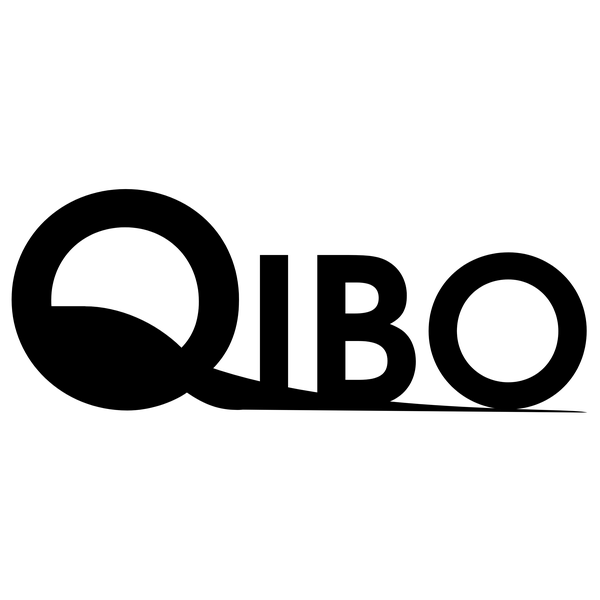
\includegraphics[width=.18\textwidth]{figures/qibo.png} 

\includegraphics[width=.18\textwidth]{figures/unimi.png} 

\includegraphics[width=.18\textwidth]{figures/cern.png}  

\includegraphics[width=.18\textwidth]{figures/qti.png}  
};
\end{tikzpicture}
}



\begin{document}


\maketitle

\begin{frame}{Working in the NISQ era}
    \begin{figure}  
    \includegraphics[width=1\textwidth]{figures/mr_research.png}
    \end{figure}
    \vspace{-0.5cm}
\end{frame}

\begin{frame}{What is \texttt{qibo}?}
\small
    \begin{figure}  
    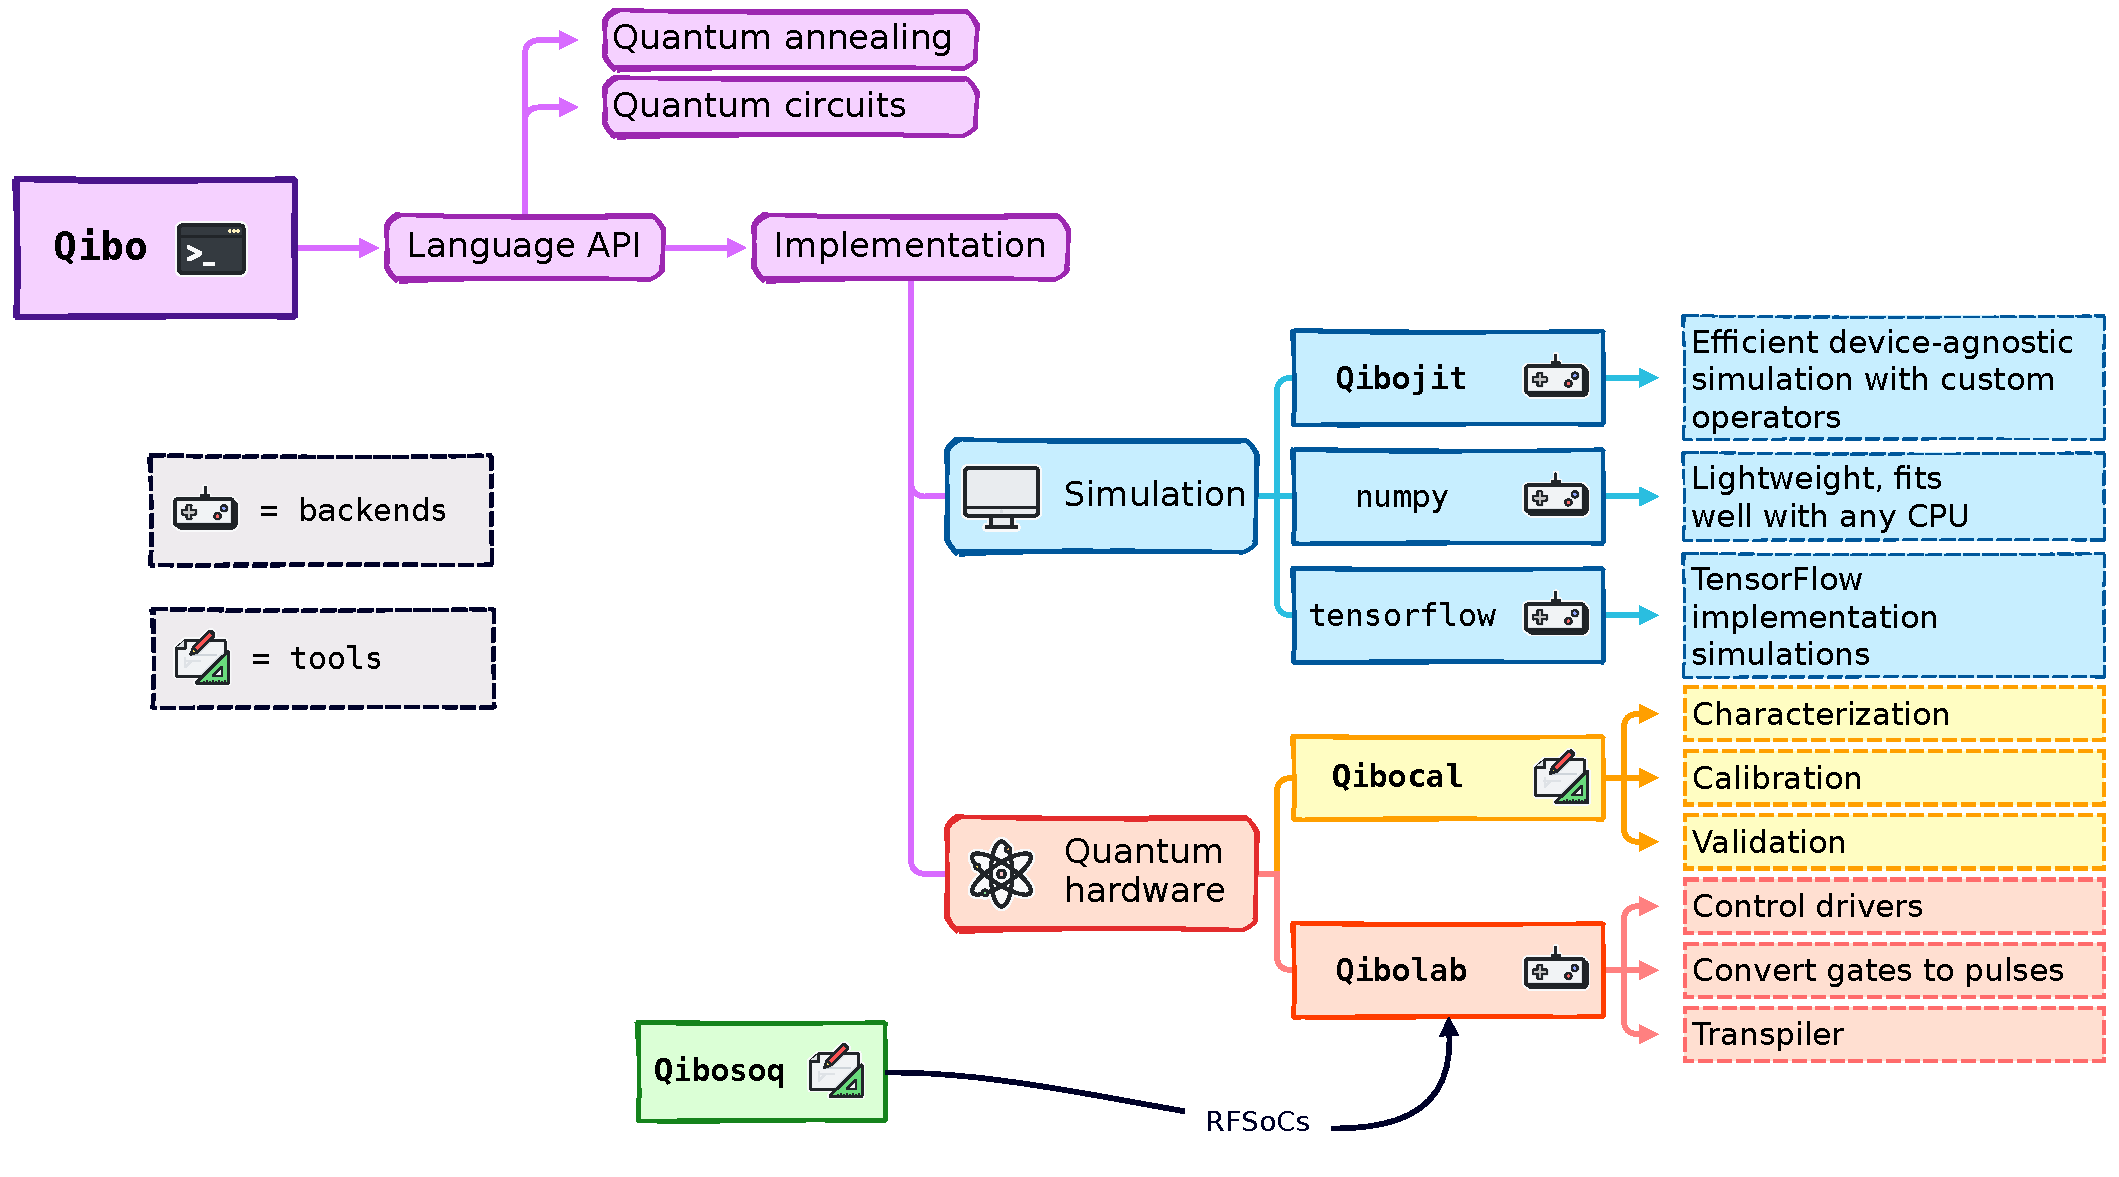
\includegraphics[width=1\textwidth]{figures/qibo_ecosystem.png}
    \end{figure}
    \vfill
    \footnotesize
    \faBook\,\,\href{https://arxiv.org/abs/2009.01845}{arXiv:2009.01845}: \textit{``Qibo: a framework for quantum simulation with hardware acceleration."}\\
\end{frame}

\section{Some features}

\begin{frame}{More about \texttt{qibojit}}
\small
\faArrowCircleRight\,\, We do state vector simulation, which solves:
\begin{equation}
\psi'(\sigma_1, ..., \sigma_n) = \sum_{\tau'}G(\tau, \tau') \psi(\sigma_1, ..., 
\tau', ..., \sigma_n),
\end{equation}
\pause
\faArrowCircleRight\,\, where the number of operations scales exponentially with $N_{qubits}$.

\pause
\faArrowCircleRight\,\, For this reason we built \texttt{qibojit} (recommended if $N_{qubits \geq 20}$):
    \begin{figure}  
    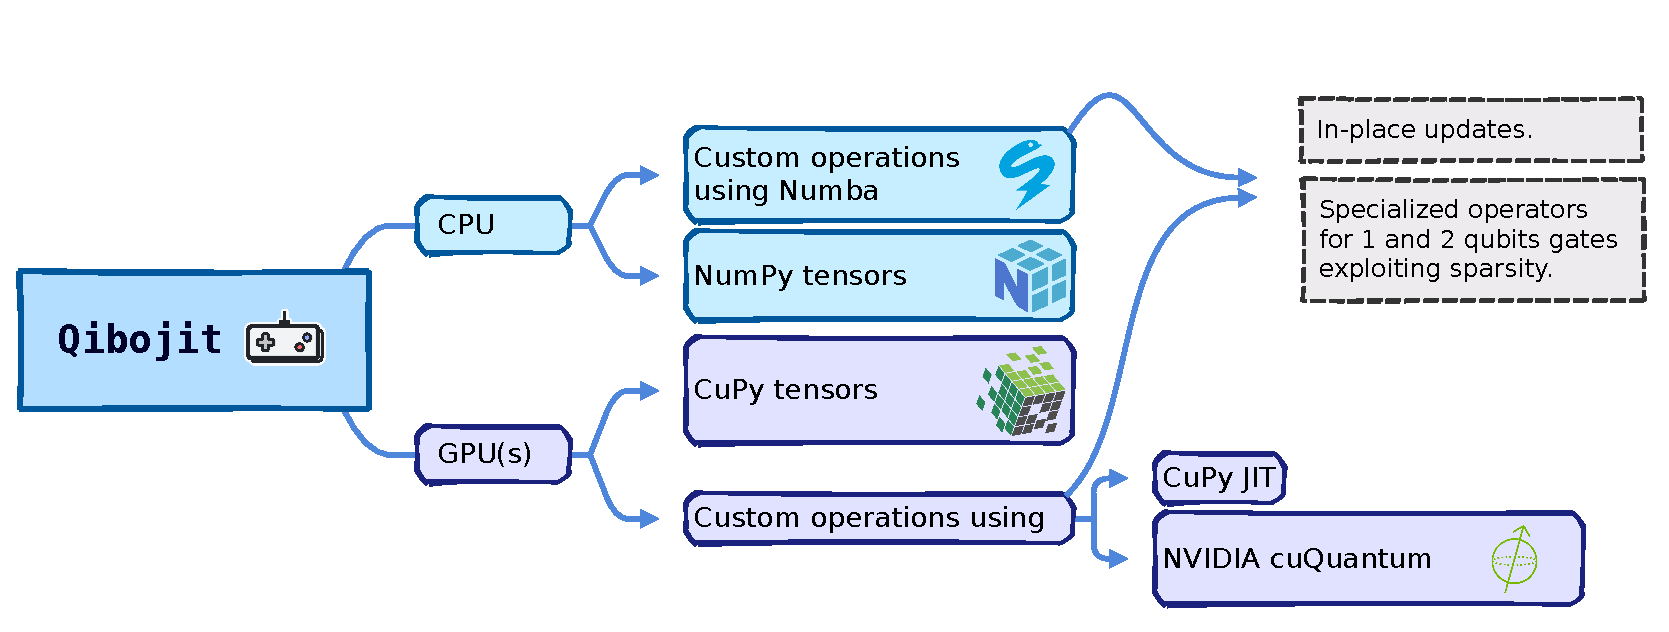
\includegraphics[width=0.9\textwidth]{figures/qibojit.png}
    \end{figure}
    \vfill
    \footnotesize
    \faBook\,\,\href{https://arxiv.org/abs/2203.08826}{arXiv:2203.08826}: \textit{``Quantum simulation with just-in-time compilation."}\\
\end{frame}

\begin{frame}{\texttt{qibojit} benchmarks}
\small
   \begin{figure}  
    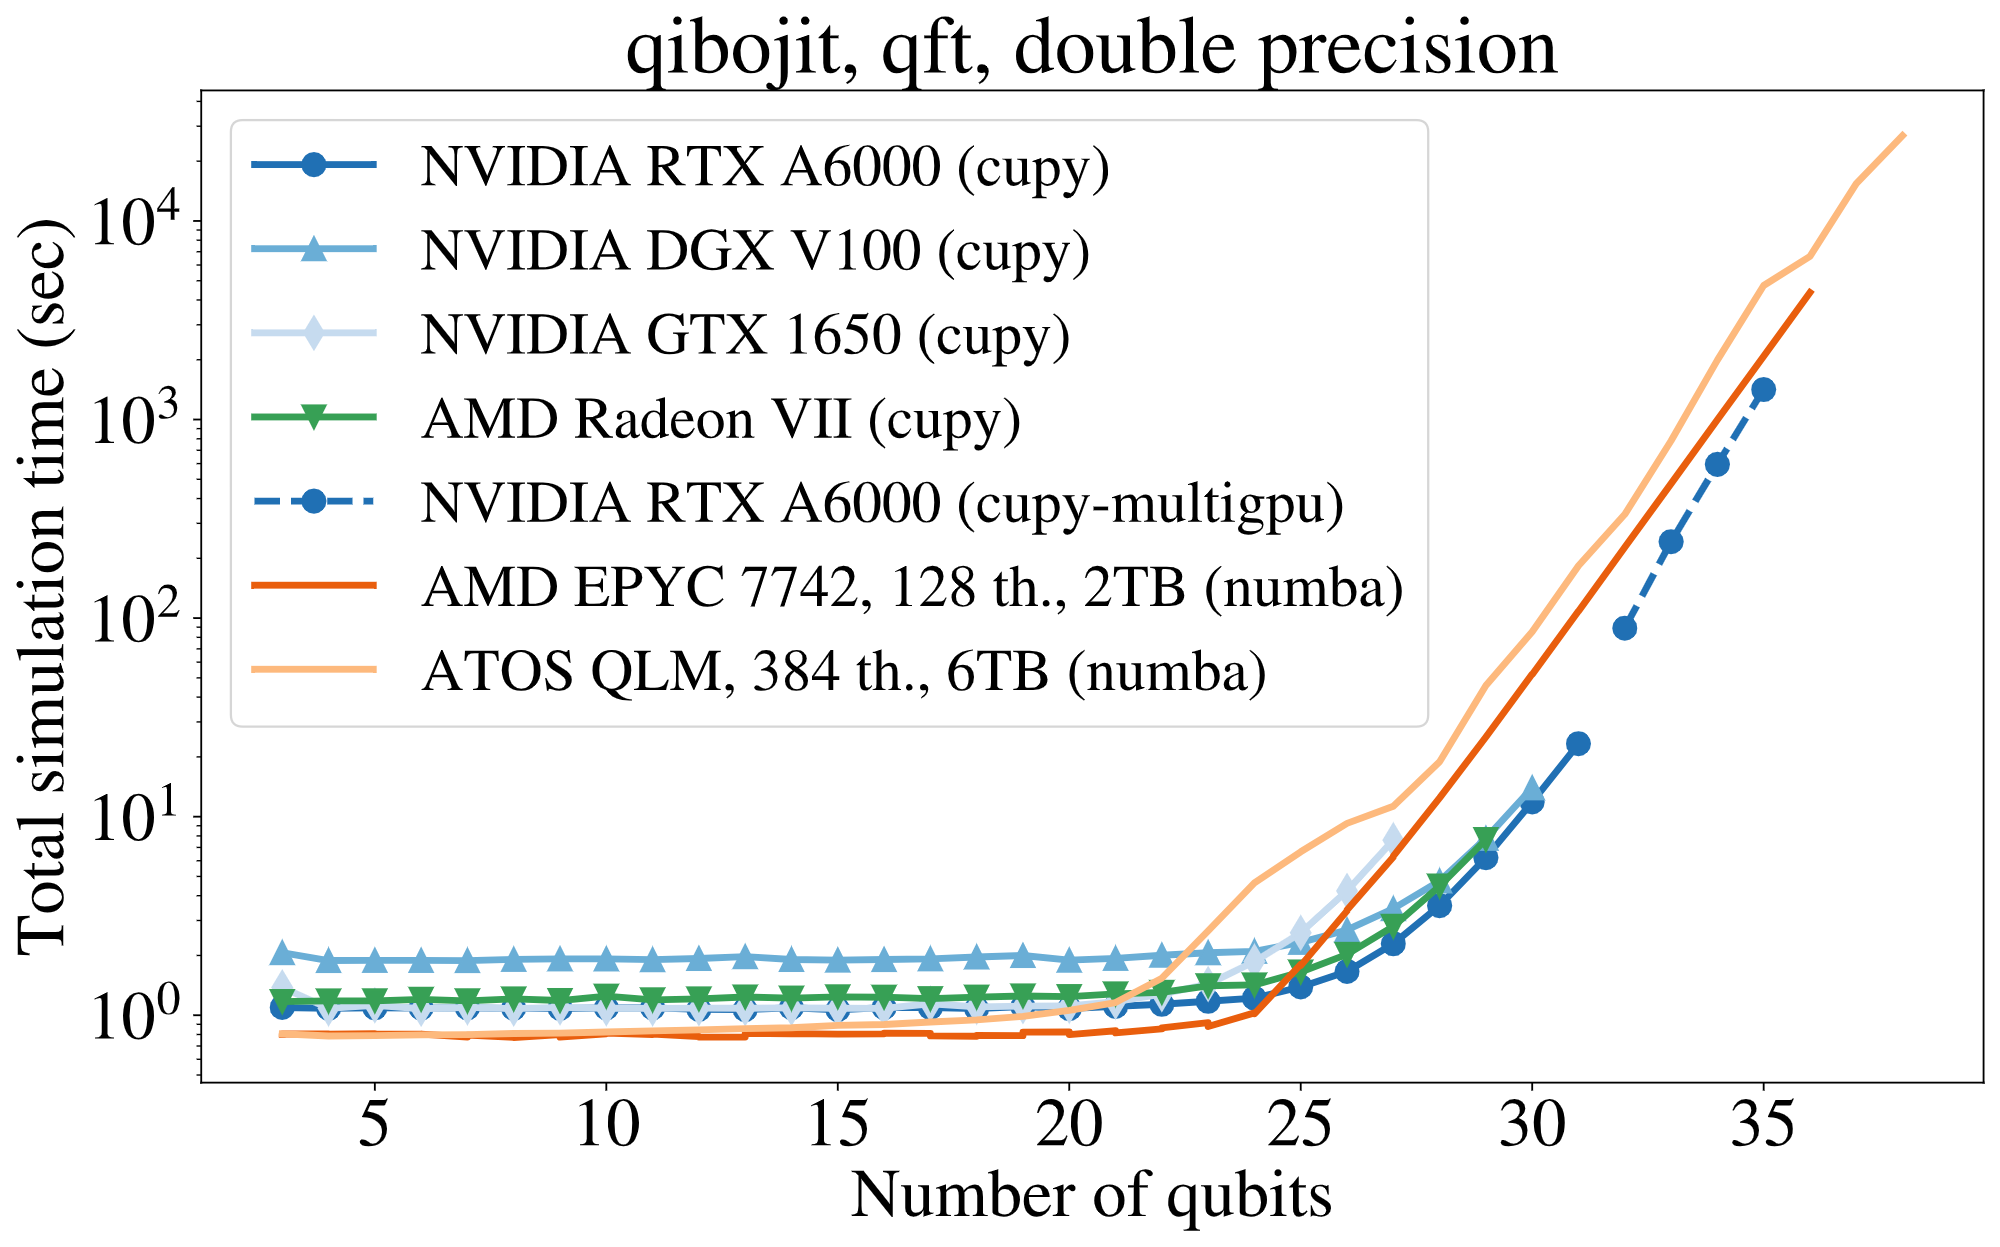
\includegraphics[width=0.85 \textwidth]{figures/qibojit-qft.png}
    \caption{Quantum Fourier Transform execution with \texttt{qibojit} backend for
    growing number of qubits.}
    \end{figure}
\end{frame}


\begin{frame}{More about quantum annealing with \texttt{qibo}}
\small
\faArrowCircleRight\,\, An \texttt{AdiabaticEvolution} model is provided, which
implements:
\begin{equation}
H_{\rm ad}(\tau; \bm{\theta}) = \bigl[ 1 - s(\tau; \bm{\theta}) \bigr] H_0 +  
s(\tau; \bm{\theta}) H_1.
\end{equation}

\pause
\faArrowCircleRight\,\, which can be used by:

\pause
\begin{itemize}[noitemsep]
\item[\faGamepad] defining $H_0$ and $H_1$ symbolically (we use 
\href{https://docs.sympy.org/latest/index.html}{\texttt{sympy}});    
\pause
\item[\faGamepad] defining a scheduling function $s(\tau; \bm{\theta})$ and a 
timestep \texttt{dt}; 
\pause
\item[\faGamepad] setting the \texttt{solver} to use for integrating Schrondiger's equation.
\pause
\item[\faGamepad] calling the \texttt{AdiabaticEvolution} object at some final time $T$.
\end{itemize}

\pause
\faArrowCircleRight\,\, This mechanism ``pushes" the state during the evolution by
sequentially executing a circuit obtained by trotterizing $H_{\rm ad}$. 

\pause
\faArrowCircleRight\,\, If \texttt{solver=="exp"}, we use the evolutionary 
operator\footnote<8->{Translated into a circuit form using the Trotter decomposition.}:
\begin{equation}
\ket{\psi(\tau = j\text{d}t)} = \prod_{j}^{\leftarrow} U_j \ket{\psi(\tau=0)} 
\end{equation}

\end{frame}

\begin{frame}{Adiabatic evolution on \texttt{qibo} backends}
\small
\begin{figure}  
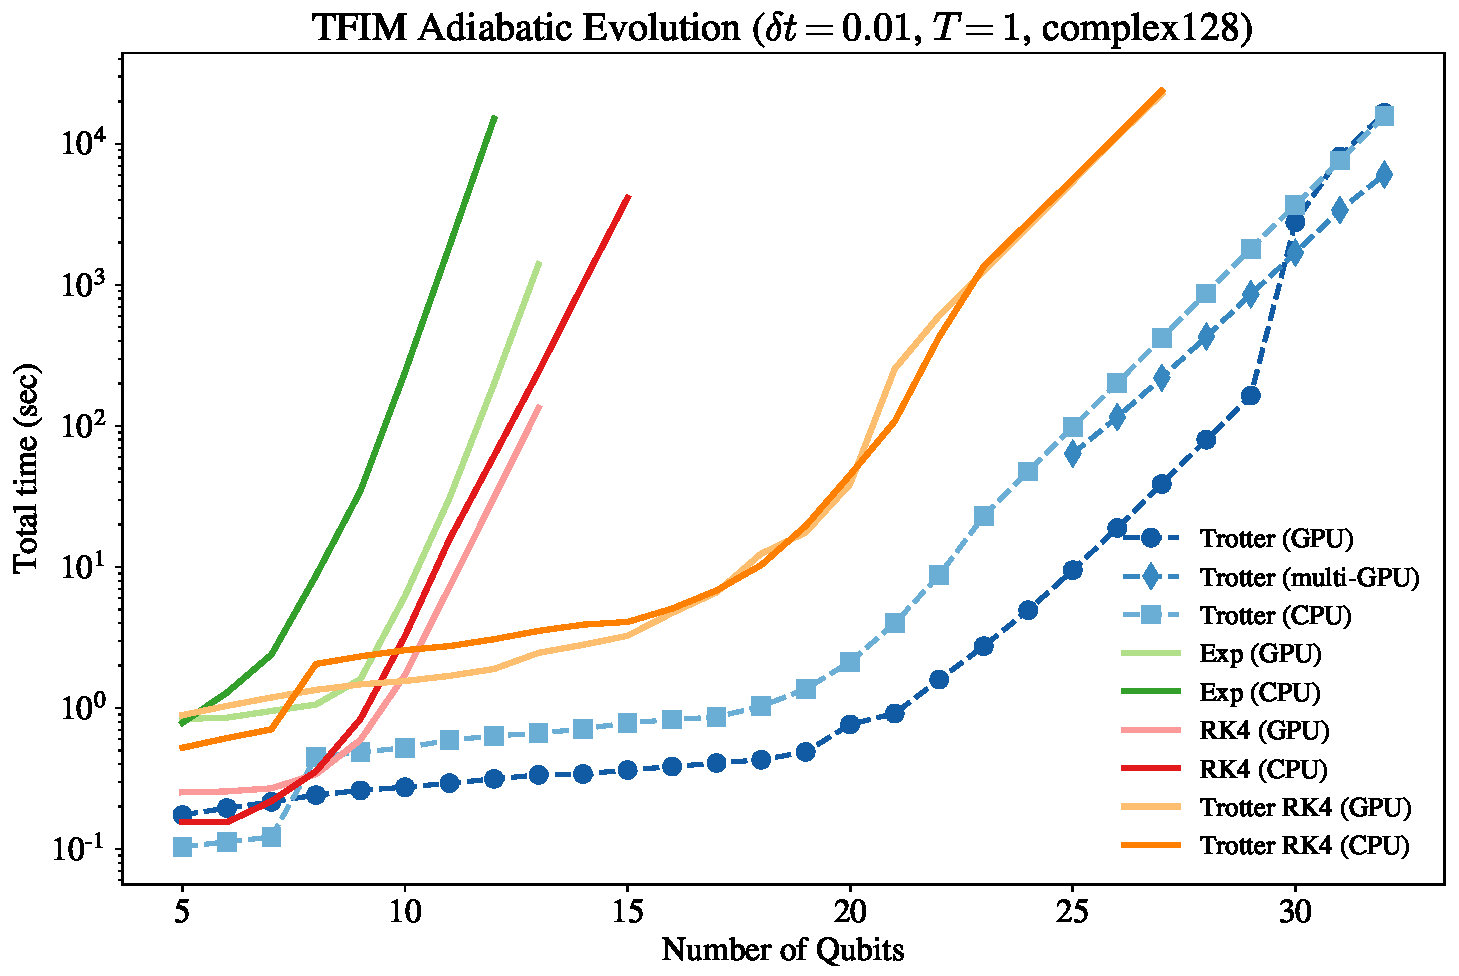
\includegraphics[width=0.75 \textwidth]{figures/adiab_evolution.pdf}
\caption{Adiabatic evolution execution with growing number of qubits and different
solvers.}
\end{figure}
\end{frame}


\section{A full-stack QML algorithm}

\begin{frame}{The theoretical idea}
\begin{figure}  
\includegraphics[width=0.85\textwidth]{figures/pdf_est.png}
\end{figure}
\end{frame}

\begin{frame}[fragile]{\texttt{SIMULATION}: fit CDF with Adiabatic Evolution (AE)}
\small

\faArrowCircleRight\,\, Given a sample $\{x\}$ and calculated its CDF values $F(x)$:
\pause
\begin{itemize}[noitemsep]
\item[\faChain] we select two hamiltonians $H_0$ and $H_1$ such that a target observable
has energy $E=0$ and $E=1$ respectively on $H_0$ and $H_1$ ground states;
\pause
\item[\faChain] we map $(x, F)\to(\tau, E)$.
\end{itemize}

\pause
\faArrowCircleRight\,\, The AE training strategy follows:
\begin{itemize}[noitemsep]
\pause
\item[1.] we run the evolution with random initial $\bm{\theta_0}$ into the scheduling;
\pause
\item[2.] we track the energy of a Pauli Z during the evolution;
\pause
\item[3.] we calculate a loss function $J_{\rm mse}$:
         $$ J_{\rm mse} = \sum_{k=1}^{N_{\rm sample}} \bigl[ E(\tau_k) - F(x_k) \bigr]^2; $$
\pause
\item[4.] we choose an optimizer to find $\bm{\theta}_{\rm best}$ which minimizes $J_{\rm mse}$.
\end{itemize} 
\pause
\vfill
\footnotesize
\faBook\,\,\href{https://arxiv.org/abs/2303.11346}{arXiv:2303.11346}: \textit{``Determining probability density functions with adiabatic quantum computing."}\\
\end{frame}

\begin{frame}[fragile]{A toy example with \texttt{nqubits=1} - starting point}
\large
\faArrowCircleRight\,\, \texttt{nparams=20}, \texttt{dt=0.1}, \texttt{final\_time=50}
, \texttt{target\_loss=None}
\begin{figure}
    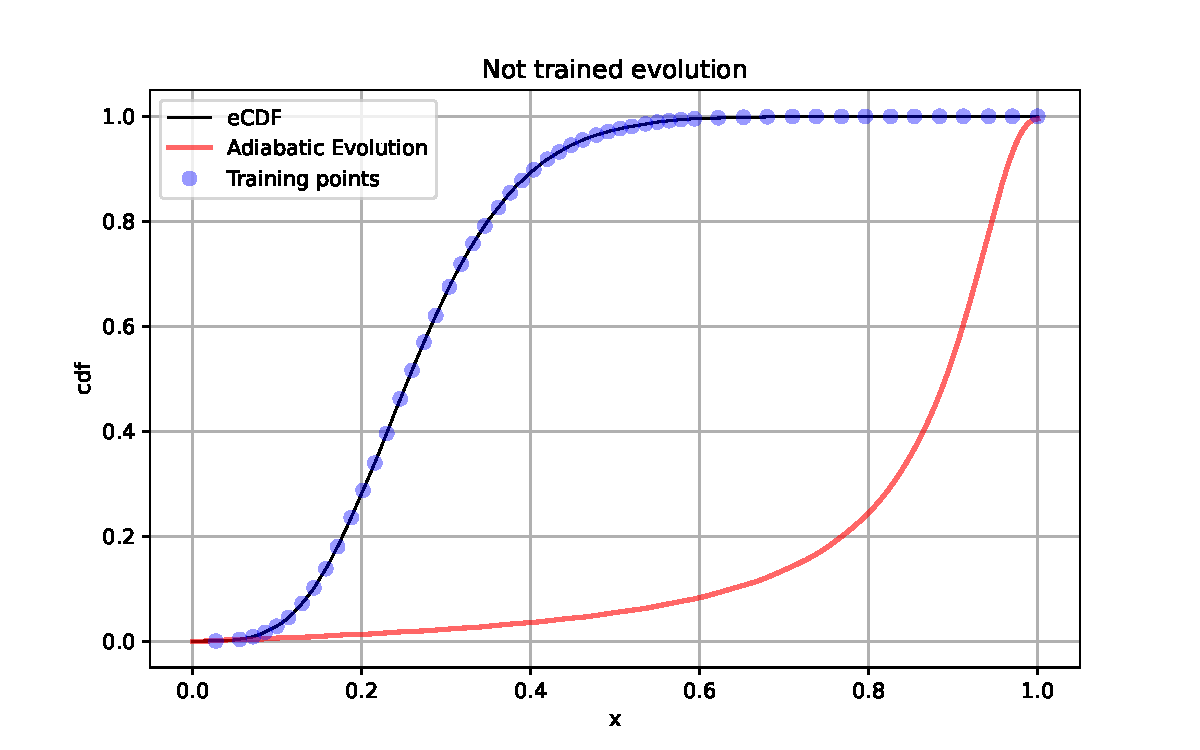
\includegraphics[width=1\textwidth]{figures/ev0.pdf}
\end{figure}
\end{frame}

\begin{frame}[fragile]{A toy example - until $J_{\rm MSE}=10^{-1}$}
\large
\faArrowCircleRight\,\, \texttt{nparams=20}, \texttt{dt=0.1}, \texttt{final\_time=50}
, \texttt{target\_loss=1e-1}
\begin{figure}
    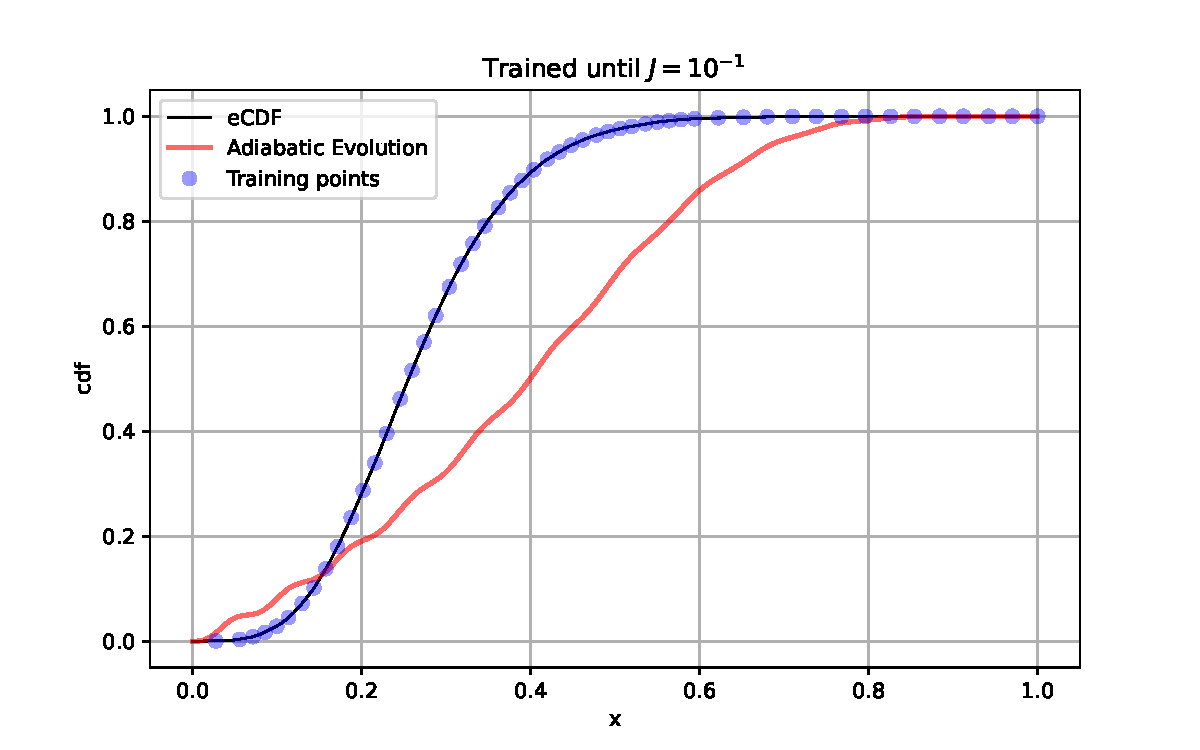
\includegraphics[width=1\textwidth]{figures/ev1.pdf}
\end{figure}
\end{frame}

\begin{frame}[fragile]{A toy example - until $J_{\rm MSE}=10^{-2}$}
\large
\faArrowCircleRight\,\, \texttt{nparams=20}, \texttt{dt=0.1}, \texttt{final\_time=50}
, \texttt{target\_loss=1e-2}
\begin{figure}
    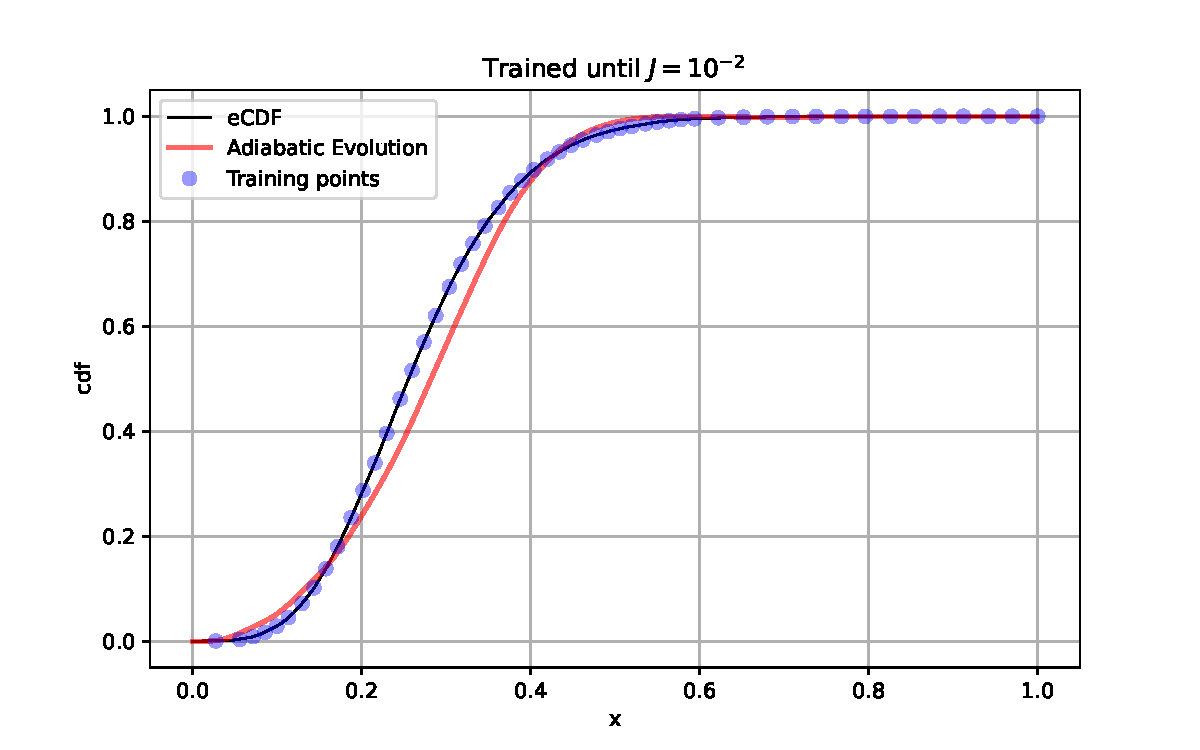
\includegraphics[width=1\textwidth]{figures/ev2.pdf}
\end{figure}
\end{frame}

\begin{frame}[fragile]{A toy example - ending at $J_{\rm MSE}=10^{-4}$}
\large
\faArrowCircleRight\,\, \texttt{nparams=20}, \texttt{dt=0.1}, \texttt{final\_time=50}
, \texttt{target\_loss=1e-4}
\begin{figure}
    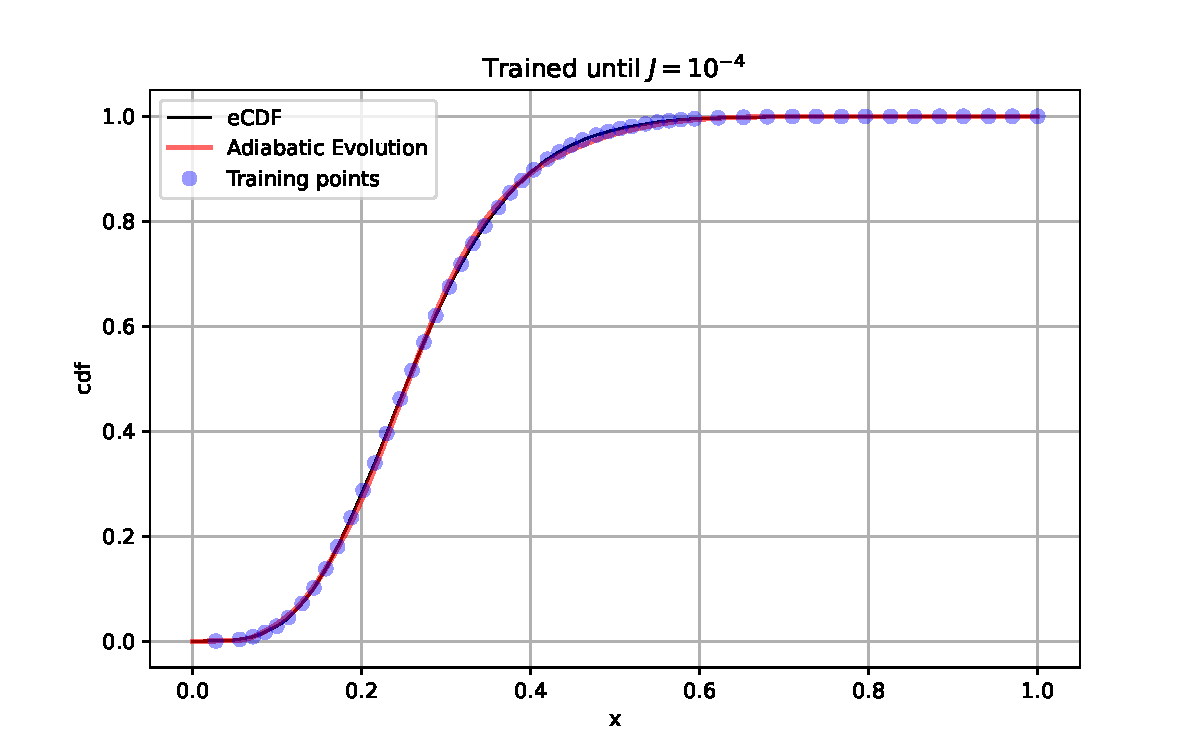
\includegraphics[width=1\textwidth]{figures/ev3.pdf}
\end{figure}
\end{frame}

\begin{frame}{\texttt{SIMULATION:} from $\{H_{\rm ad}\}$ to a circuit and derivate!}
\small
\pause
\faArrowCircleRight\,\, Firstly, we did some calculations and approximations in order to:
\pause
\begin{itemize}[noitemsep]
\item[1.] translate the Hamiltonians' sequence into a single unitary:
$$\prod_{j=1}^{n} e^{-i H_{j}\text{d}t} \to \mathcal{U}(t);$$
\pause 
\item[2.] translate this unitary in a sequence of rotational gates:
$$ \mathcal{U}(t) = R_z(\theta_1)R_x(\theta_2)R_z(\theta_3) \qquad \text{with}\,\, \theta_i \equiv \theta_i(t).$$
\end{itemize}
\pause 
\faArrowCircleRight\,\, Then, we derivate the expected values using parameter shift rule
and chain rule.
\pause 
\begin{multicols}{2}
\begin{figure}
    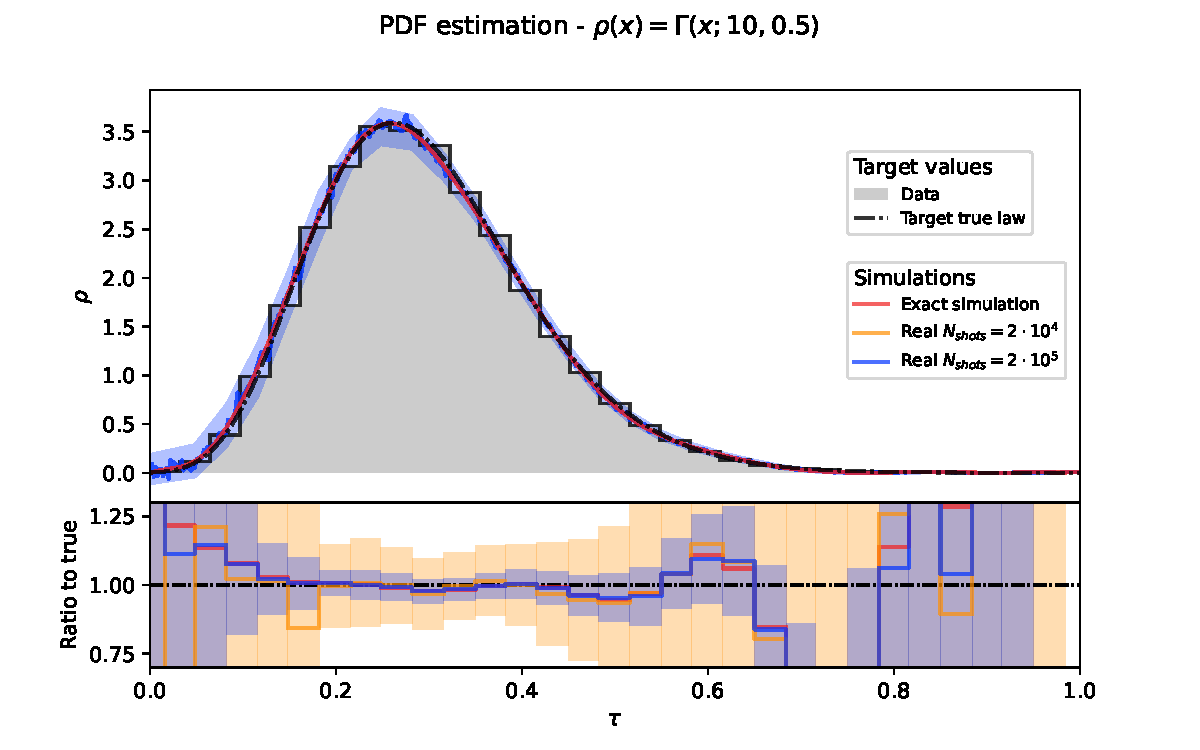
\includegraphics[width=0.5\textwidth]{figures/PDF_gamma_25_20_200000.pdf}
\end{figure}
\begin{figure}
    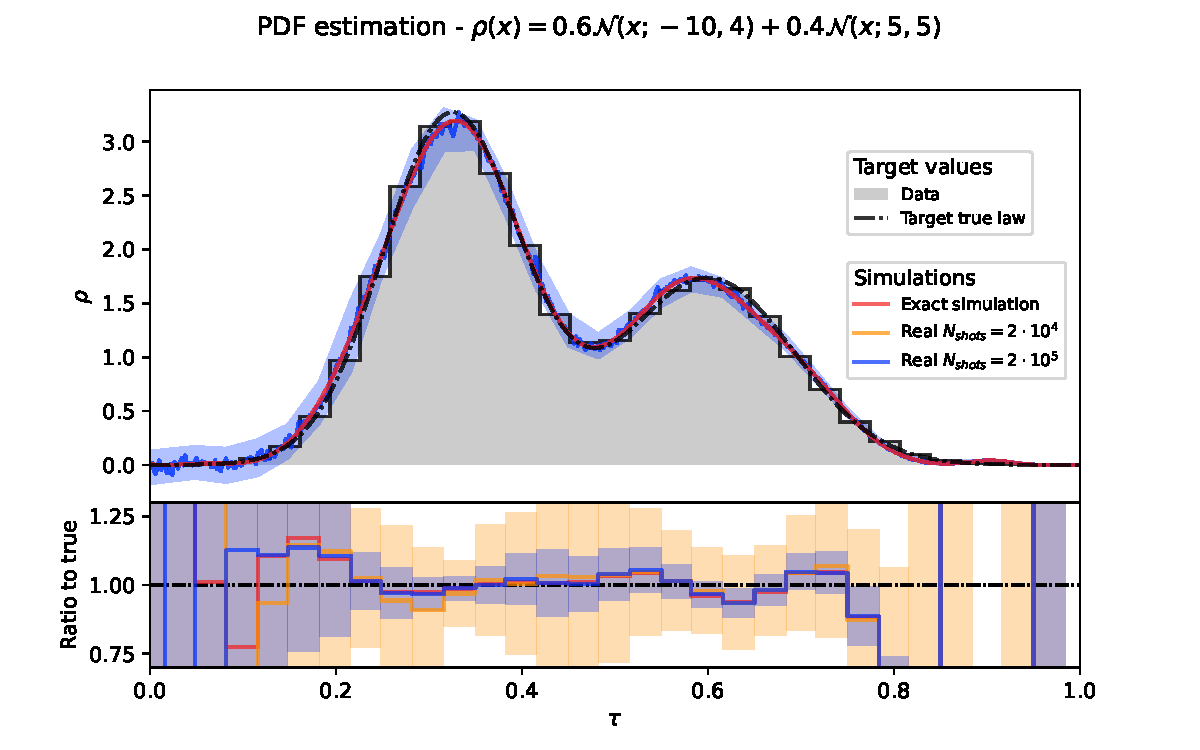
\includegraphics[width=0.5\textwidth]{figures/PDF_gauss_30_20_200000.pdf}
\end{figure}
\end{multicols}
\end{frame}

\section{Hardware deployment}

\begin{frame}{\texttt{EXECUTION:} running on the hardware}
\small
\faArrowCircleRight\,\, \texttt{qibo} is hardware-agnostic!
\pause

\faArrowCircleRight\,\, We defined an abstract \texttt{Platform} object, which can
be selected via \texttt{set\_backend("qibolab", platform="my\_platform")}. 
\begin{figure}
    \includegraphics[width=0.8\textwidth]{figures/qibolab.png}
\end{figure}

\pause
\faArrowCircleRight\,\, Some labs are already using \texttt{qibo}:
\begin{multicols}{4}
\begin{figure}
    \centering 
    
\includegraphics[width=0.12\textwidth]{figures/infn.png}
\end{figure}
\begin{figure}
    \centering 
    
\includegraphics[width=0.12\textwidth]{figures/tii.png}
\end{figure}
\begin{figure}
    \centering 
    
\includegraphics[width=0.12\textwidth]{figures/cqt.png}
\end{figure}
\begin{figure}
    \centering 
    
\includegraphics[width=0.12\textwidth]{figures/bsc.jpg}
\end{figure}
\end{multicols}
\pause
\footnotesize
\faBook\,\,\href{https://arxiv.org/abs/2202.07017}{arXiv:2202.07017}: \textit{``An open-source modular framework for quantum computing."}
\faBook\,\,\href{https://arxiv.org/abs/2112.02933}{arXiv:2112.02933}: \textit{``ICARUS-Q: Integrated Control and Readout Unit for Scalable Quantum Processors"}\\

\end{frame}

\begin{frame}{\texttt{qibolab} is not enough!}

\small

\faArrowCircleRight\,\, Each quantum control routine is useless if the sequences
of pulses are not well calibrated with the single qubit.
\pause

\faArrowCircleRight\,\, For this reason, \texttt{qibocal} was born: a module for
quantum calibration and verification.

    \begin{figure}  
    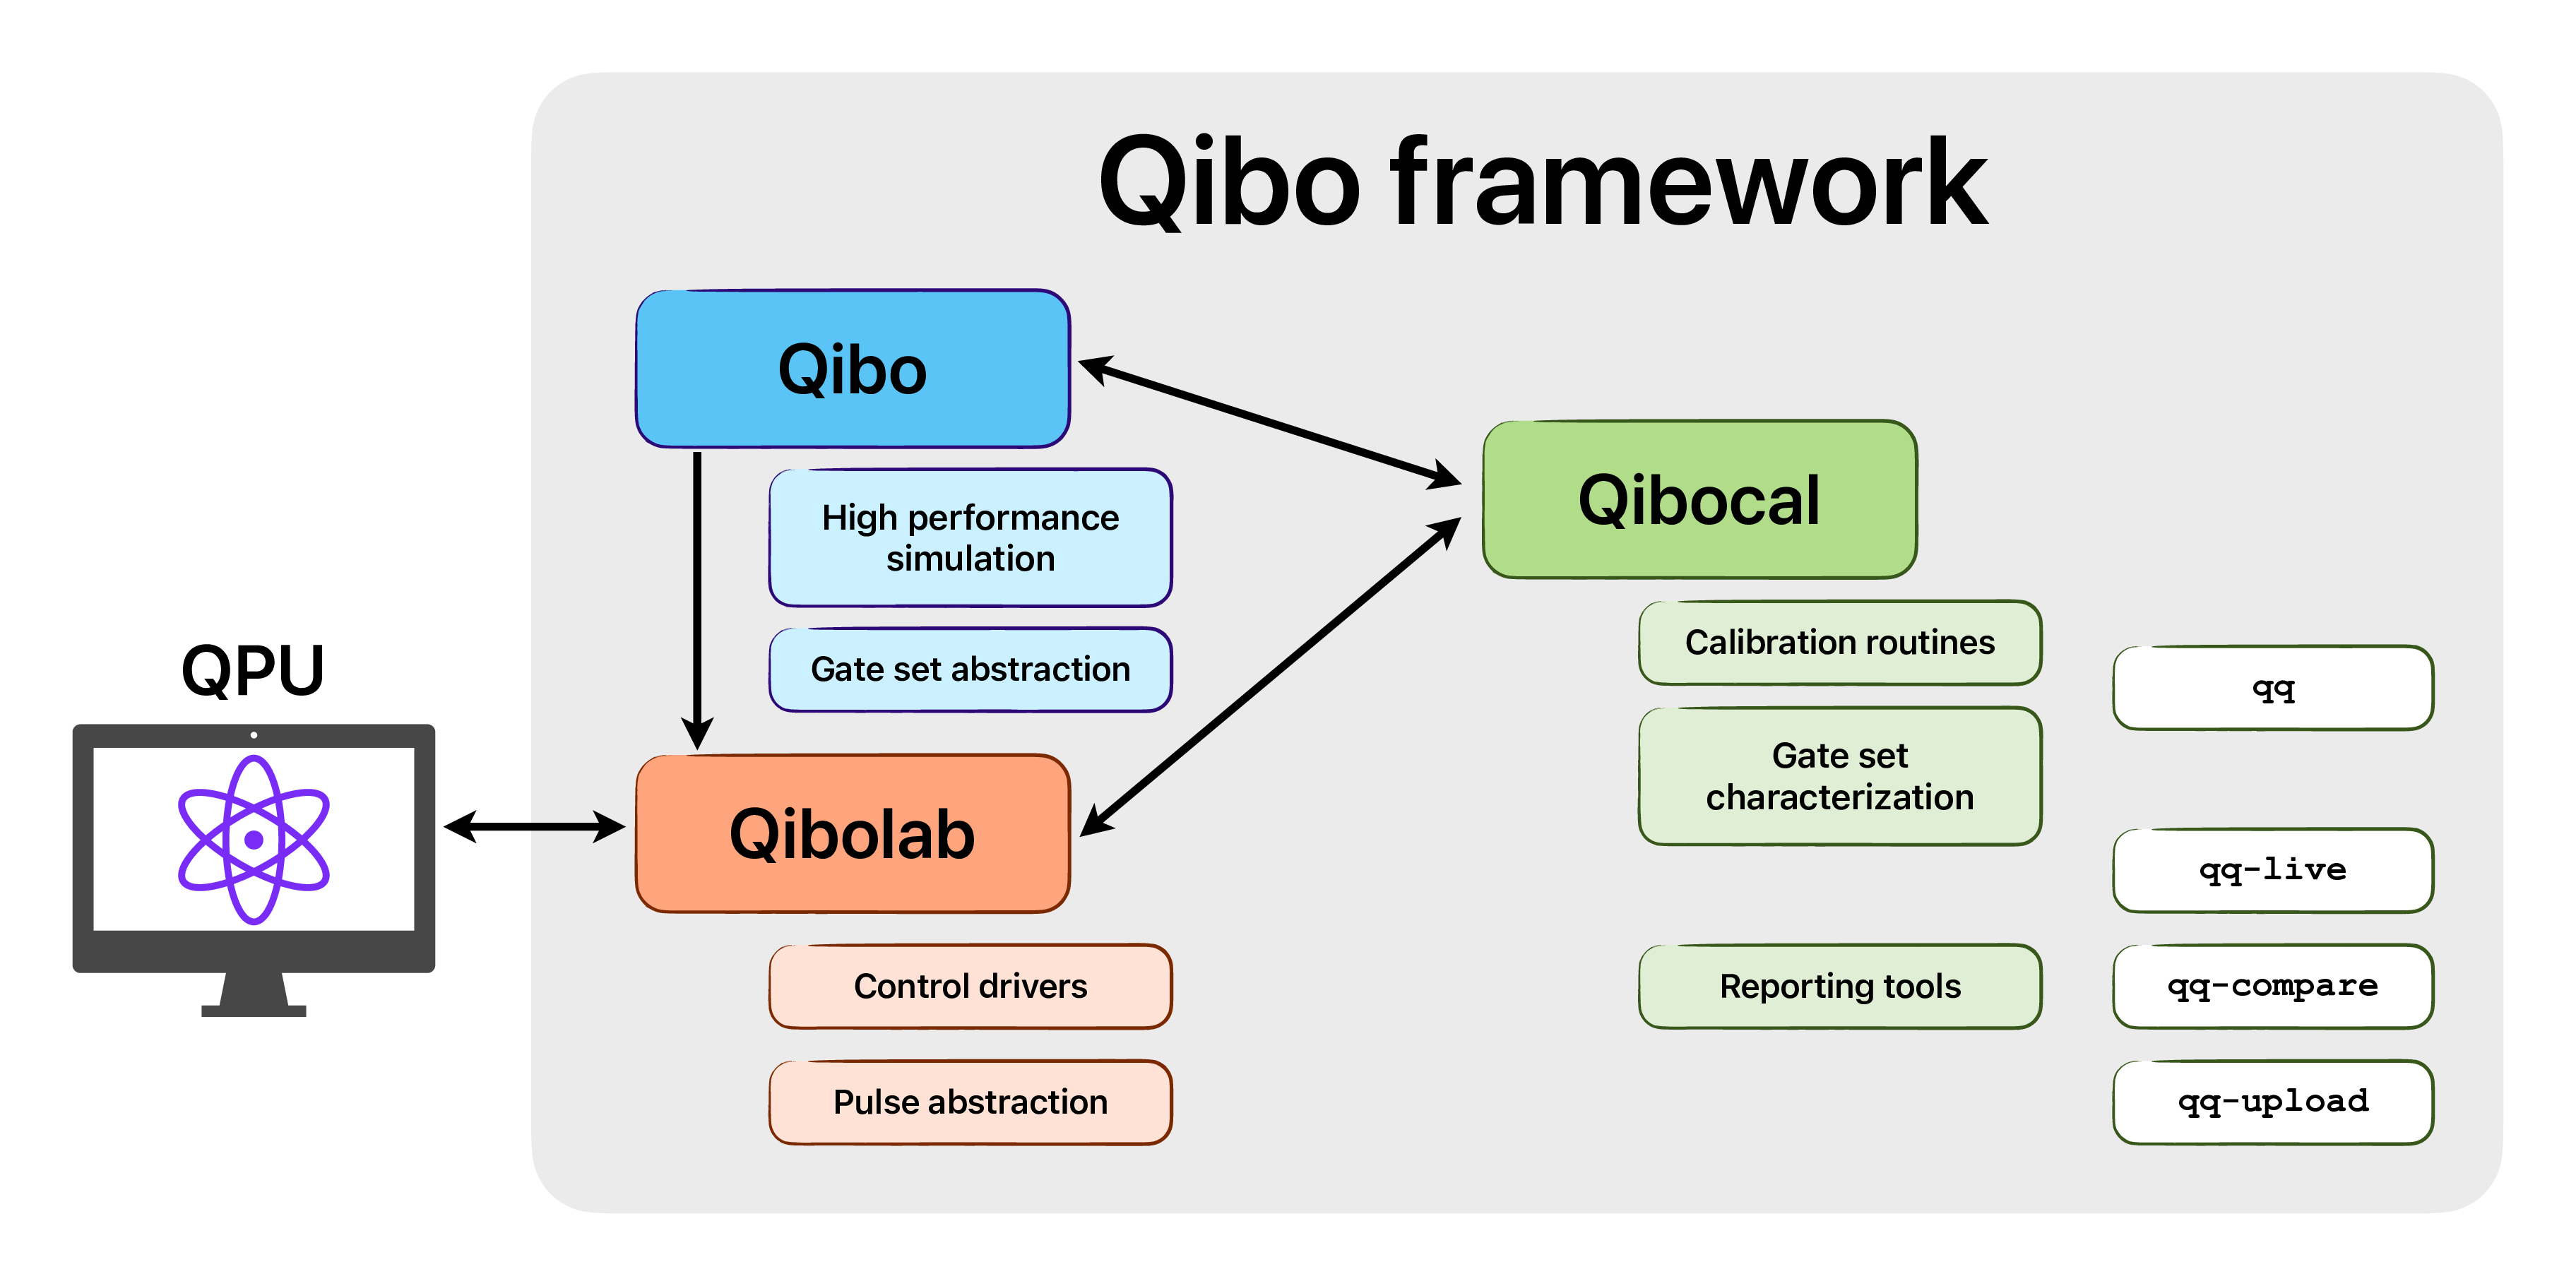
\includegraphics[width=1\textwidth]{figures/qibocal_in.png}
    \end{figure}
\pause

\footnotesize
\faBook\,\,\href{https://arxiv.org/abs/2303.10397}{arXiv:2303.10397}: \textit{``Towards an open-source framework to perform quantum calibration and characterization."}
\end{frame}


\begin{frame}{The importance of \texttt{qibocal}}
\small 
\begin{figure}  
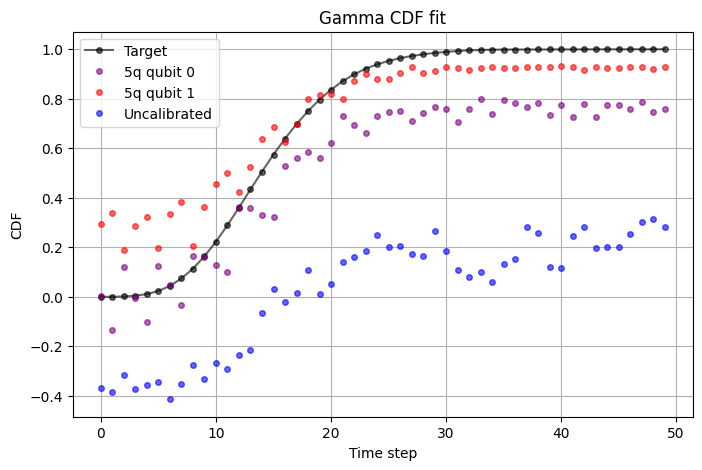
\includegraphics[width=0.7\textwidth]{figures/cal_fit.png}
\caption{Different qubits requires different calibration and leads to different results.}
\end{figure}
\pause
\faArrowCircleRight\,\, Open questions:
\pause
\begin{itemize}[noitemsep]
\item[\faHandPointerO] what if the entire training is performed on a NISQ device? \textit{are
the results self-resistent to the noise?}
\pause
\item[\faHandPeaceO] what needed for improving results on the hardware? 
\end{itemize}
\end{frame}

\section{\faHandPointerO:\,\, what if we train on hardware?}



\begin{frame}{The theoretical idea}
\small

\faArrowCircleRight\,\,Following \href{https://arxiv.org/abs/1907.02085}{\textit{Pérez-Salinas et al.}} 
procedure, we can build a \textit{universal quantum regressor}
for approximating $y=f(x)$. The model can be:
\pause
    \begin{figure}  
    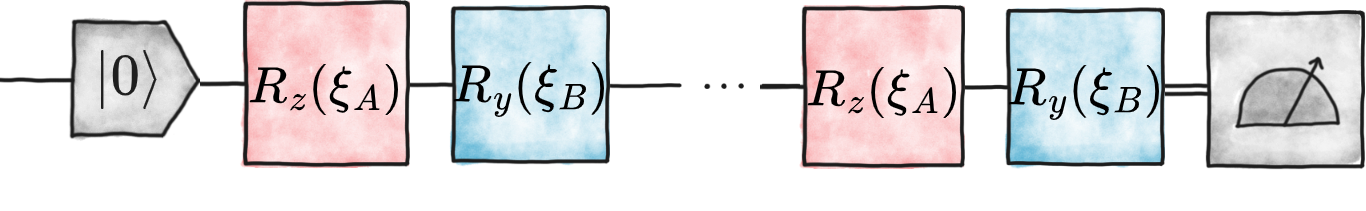
\includegraphics[width=0.85\textwidth]{figures/qpdf.png}
    \caption{Here $\xi_A= \theta_1x+\theta_2$ and $\xi_B = \theta_3x + \theta_4$.}
    \end{figure}
\pause
\faArrowCircleRight\,\, and then use some $E[\hat{O}]$ as predictor:
\begin{equation}
y_{pred} = \braket{0 | \mathcal{C}^{\dagger} (x; \bm{\theta}) \hat{O} \,
\mathcal{C} (x; \bm{\theta}) | 0}.
\end{equation}
\pause
\faArrowCircleRight\,\, Using the parameter-shift rule, we can perform a Stochastic
Gradient Descent (SGD) on the hardware.
\pause

\vfill
\footnotesize
\faBook\,\,\href{https://arxiv.org/abs/2210.10787}{	arXiv:2210.10787}: \textit{``A quantum analytical Adam descent through parameter shift rule using Qibo."}

\end{frame}

\begin{frame}{Simulation results}

\begin{multicols}{2}
\begin{figure}
    \centering 
    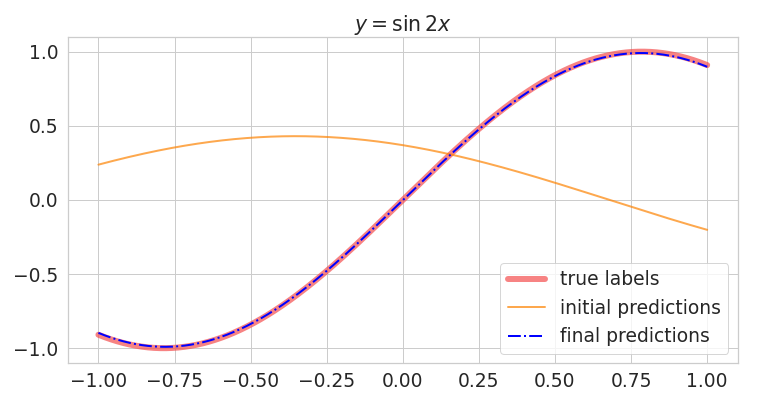
\includegraphics[width=0.5\textwidth]{figures/f0.png}
\end{figure}
\begin{figure}
    \centering 
    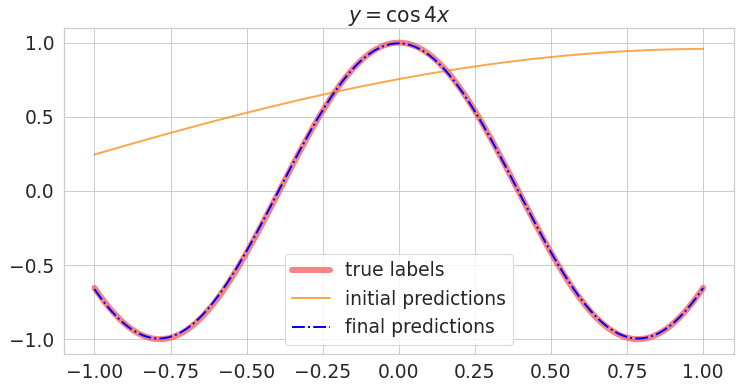
\includegraphics[width=0.5\textwidth]{figures/f1.png}
\end{figure}
\end{multicols}  
\begin{multicols}{2}
\begin{figure}
    \centering 
    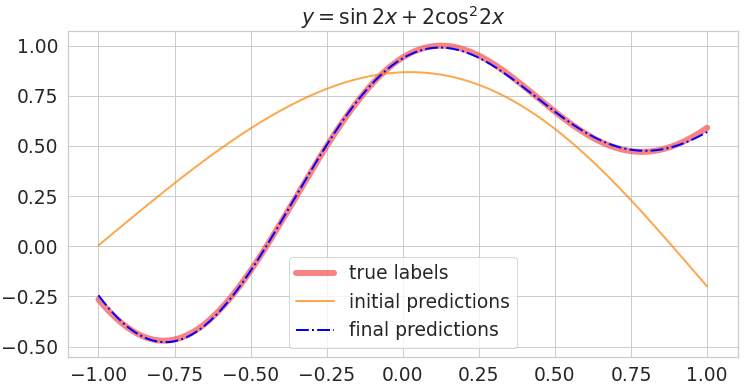
\includegraphics[width=0.5\textwidth]{figures/f2.png}
\end{figure}
\begin{figure}
    \centering 
    \includegraphics[width=0.5\textwidth]{figures/f3.png}
\end{figure}
\end{multicols}

\end{frame}

\begin{frame}{Run on the hardware}
\small

    \begin{figure}  
    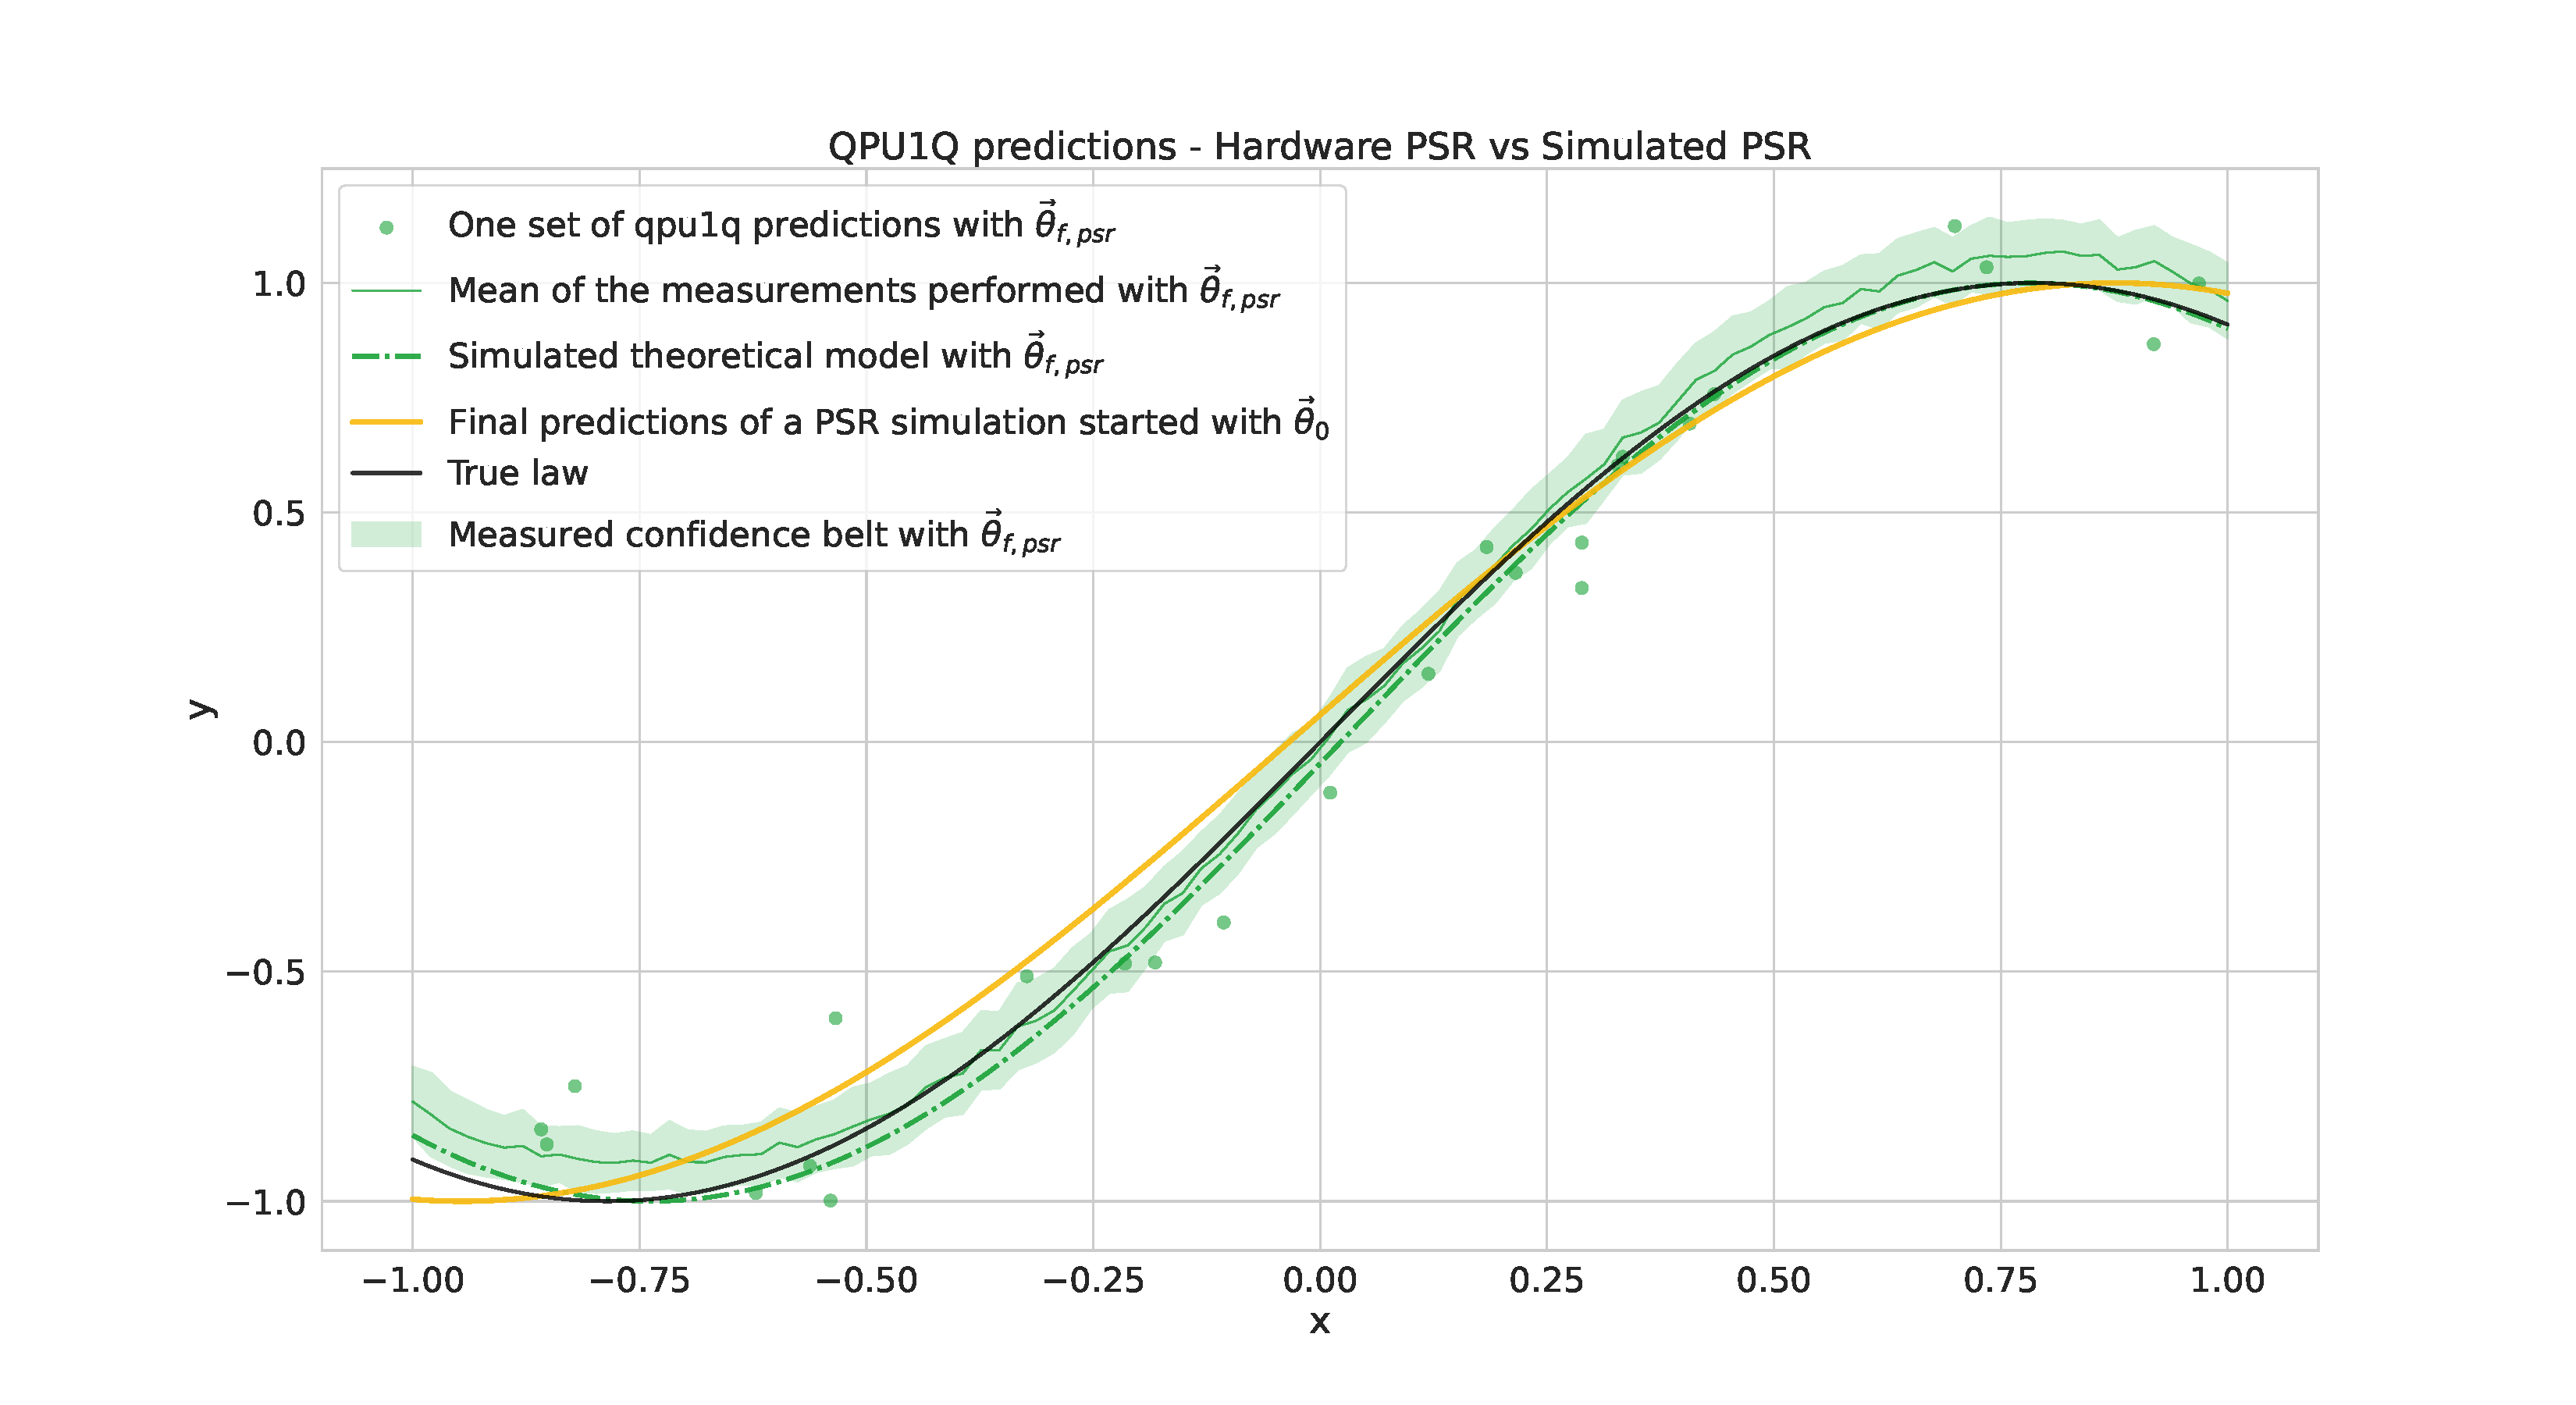
\includegraphics[width=1\textwidth]{figures/qpu1.pdf}
    \caption{Batch Gradient Descent on the hardware, with gradients evaluated 
    via Parameter-Shift Rule. We take $100$ points $\{x_j\}$ in the range $[-1,1]$ and we make 
    $100$ predictions for each $x_j$. Mean and standard deviation are used for 
    determining the estimations and the confidend belt.}
    \end{figure}

\end{frame}

\begin{frame}{Run on the hardware}
\small

    \begin{figure}  
    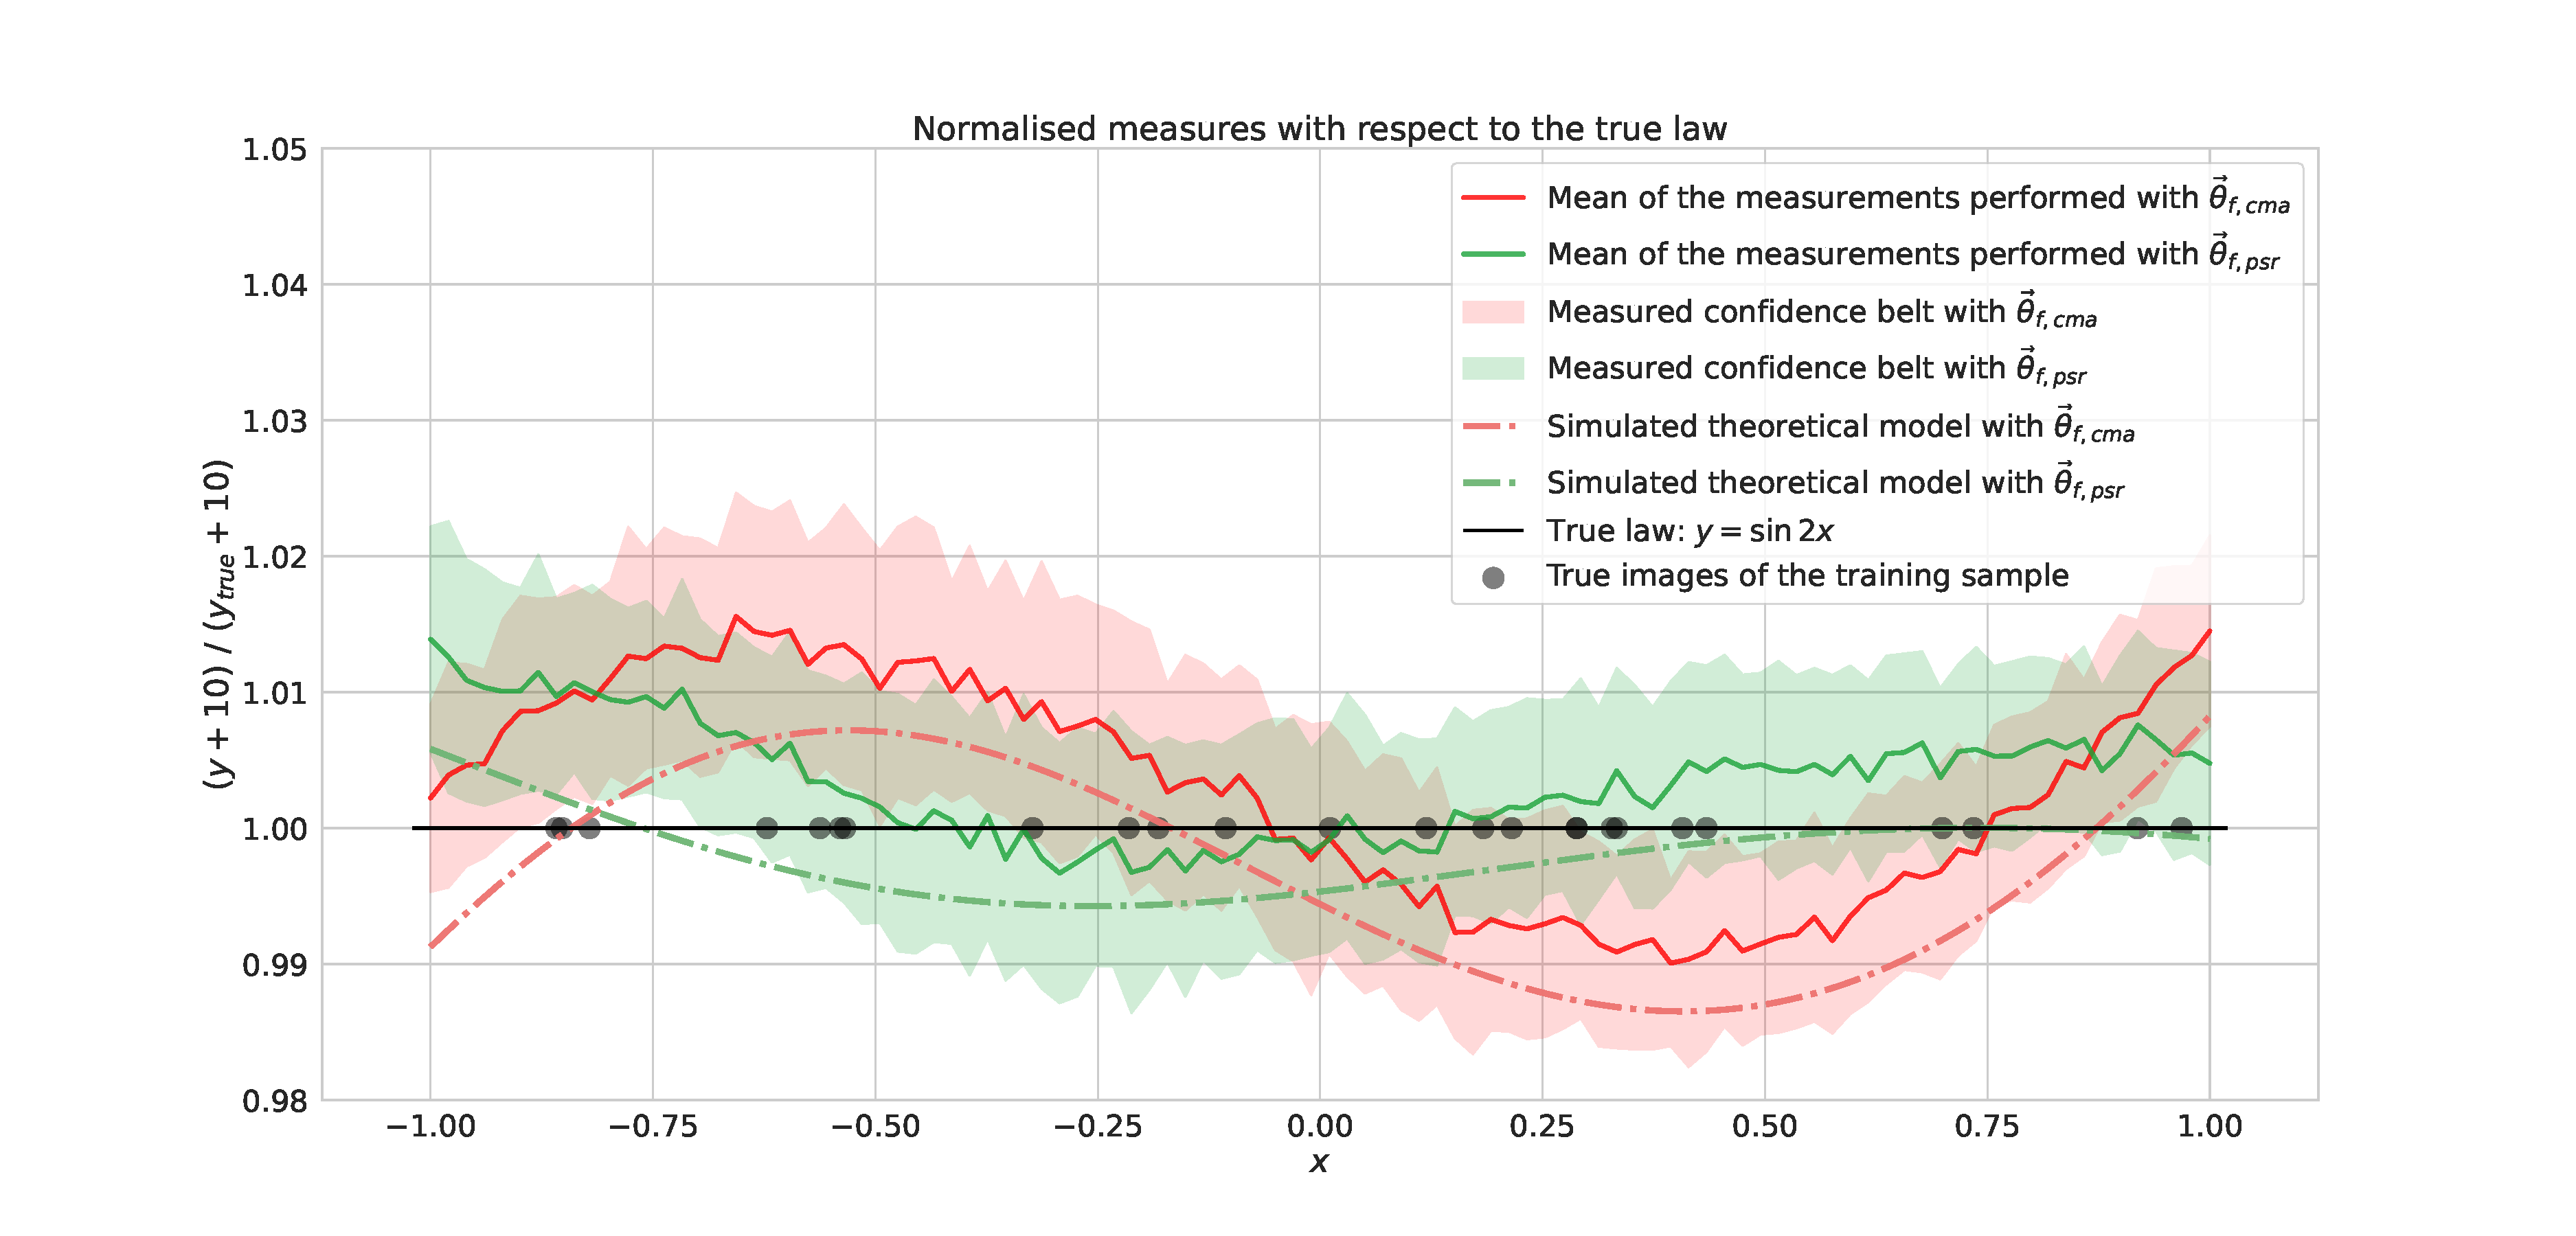
\includegraphics[width=1\textwidth]{figures/ratio_plot.pdf}
    \caption{Normalised results of the SGD (green line) compared with true law 
    and a genetic optimizer (red line).}
    \end{figure}

    \pause
    \begin{itemize}[noitemsep]
    \item[\faThumbsUp] the full-stack framework works! comparable with a genetic algorithm;
    \pause
    \item[\faThumbsDown] we can tackle only easy problems: it is slow;
    \pause
    \item[\faMehO] no mitigation: have been the errors absorbed into the optimization?
    \end{itemize}

\end{frame}

\section{\faHandPeaceO:\,\, how to get noise resistance?}

\begin{frame}{\texttt{SIMULATION}}
\small
\faArrowCircleRight\,\, We want to reproduce the $u$ quark PDF fit of \href{https://arxiv.org/abs/2011.13934}{\textit{Pérez-Salinas et al}}.

\pause
\faArrowCircleRight\,\, We apply error mitigation techniques\footnote{
    We used Zero Noise Extrapolation (ZNE) and Clifford Data Regresssion (CDR).
} during
a QML training! 
\pause
    \begin{figure}
    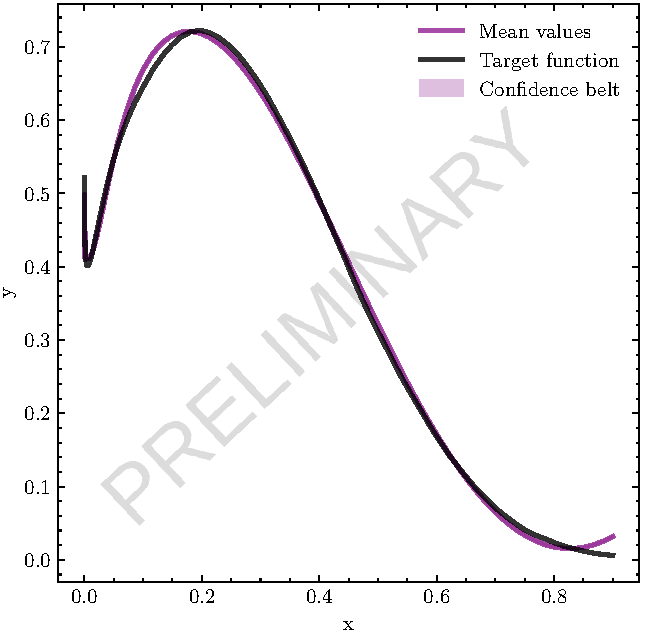
\includegraphics[height=3cm, width=0.33\textwidth]{figures/exact.pdf}%
    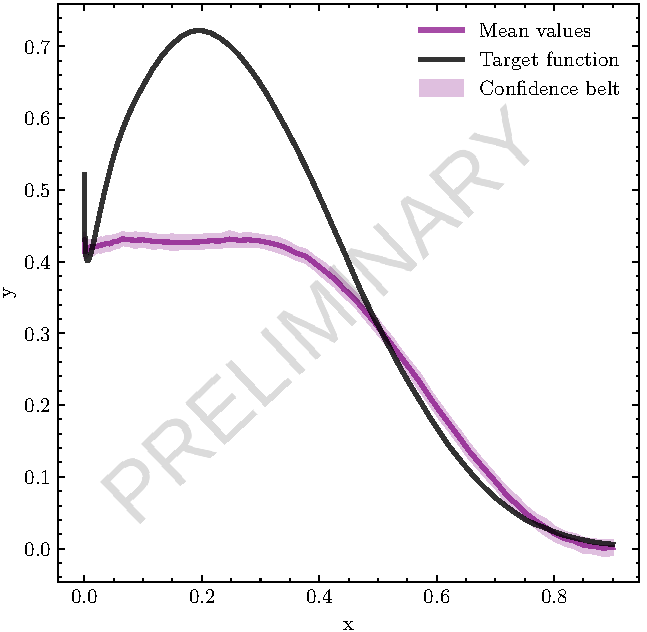
\includegraphics[height=3cm, width=0.33\textwidth]{figures/noisy.pdf}%
    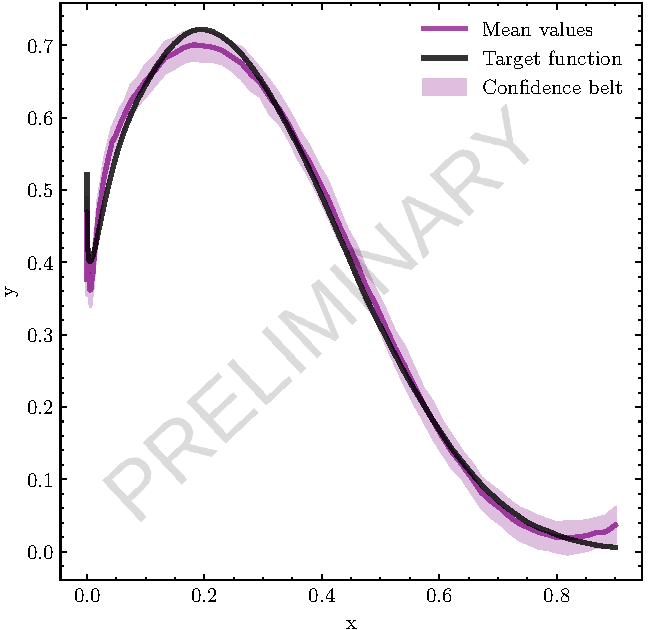
\includegraphics[height=3cm, width=0.33\textwidth]{figures/mitigated.pdf}%
    \caption{PDF fit performed with different levels of noisy simulation. 
    From left to right, exact simulation, noisy simulation, noisy simulation 
    applying error mitigation to the predictions.}
    \end{figure}
\pause
\faArrowCircleRight\,\, Run on the hardware upcoming!
\end{frame}

\section{Conclusions}

\begin{frame}{Conclusions}
\small

\faArrowCircleRight\,\, I am excited to be part of the \texttt{qibo} team 
and to share it with you:
\pause
\begin{itemize}[noitemsep]
    \item[\faCogs] it's a perfect environment to tackle QML problems at $360$°;
    \pause
    \item[\faGroup] is based on a research-centred network, that we would like to grow more 
    and more.
\end{itemize}
\pause
\begin{figure}  
\includegraphics[width=0.75\textwidth]{figures/mr_research.png}
\end{figure}

\pause
\vfill
\faGithub\,\, code is open-source \href{https://github.com/qiboteam/qibo}{here}: feel free to make your own contribution!\\
\faBook\,\, Have a look to our \href{https://qibo.science/}{documentation}.
\end{frame}



\end{document}
